% ========== Appendix C
 
\chapter{Inter- and Intra-Frontier Comparison Metrics}
\label{chap:appCComparisonMetrics}
This chapter describes in more detail the metrics used to compare the frontiers generated by solving the multi-objective model described in \S \ref{sec:model}. The metrics are broken up into two groups. \textit{Inter-frontier comparison metrics} are those metrics that quantify some feature of a frontier. That is, the metric has only a single value per frontier. These metrics may be used either alone or with other metrics to make comparisons at the frontier level. \textit{Intra-frontier comparison metrics} are those metrics that quantify some feature within a frontier. There may be multiple values of this metric per frontier, depending on the metric and the number of objectives. These metrics may be used either alone or with other metrics to make comparisons at the objective (or ecosystem service) level.

\section{Inter-Frontier Comparison Metrics}
\label{sec:emoMetrics}
Researchers in the field of EMO develop algorithms to generate a set of non-dominated solutions that best represents the true Pareto-optimal frontier \cite{deb2001multi}. To test their algorithms, they solve a benchmark multi-objective optimization problem and compare their resulting frontiers to the known Pareto front for that problem \cite{knowles2002metrics}. There is no assurance of optimality of the solutions derived using these algorithms, so they require a means of comparing the resulting frontiers to determine if one algorithm produces a ``better'' non-dominated frontier than another. Zitzler et al. provide a review of comparison methods \cite{zitzler2003performance}. These methods aim to quantify certain traits about a frontier that can be used to measure their success in approximation of the true frontier.

When necessary, the normalization of the objective space is such that all objectives are maximized, and each frontier is contained within the unit hypercube. That is, each objective is bounded between 0 and 1, yielding a frontier bounded by $[0,1]^N$. Defining the nadir solution $\mathbf{z}_{\text{nad}}$ of a frontier of points $z \in Z$ as the objective vector with components
\begin{align}
\mathbf{z}_{\text{nad}}^i = \inf_{z} \{ z^i \} \quad \forall 1 \le i \le N
\end{align}
and the ideal solution as the objective vector with components
\begin{align}
\mathbf{z}_{\text{ideal}}^i = \sup_{z} \{ z^i \} \quad \forall 1 \le i \le N
\end{align}
then under my normalization, the nadir solution is the origin and the ideal solution is the $N$-dimensional vector of ones $\mathbf{1}_N$.

The definitions of dominance terms used here are in Table \ref{tab:dominanceRelations}.

\begin{table}[ht]
\centering
\resizebox{\textwidth}{!}{%
\begin{tabular}{|p{.2\linewidth}|p{.1\linewidth}|p{.3\linewidth}|p{.1\linewidth}|p{.3\linewidth}|}
\hline
\textbf{Relation}           & \multicolumn{2}{c|}{\textbf{Solutions}}                                                                                                                                                                          & \multicolumn{2}{c|}{\textbf{Frontiers}}                                                                                                     \\ \hline
Strictly dominates & $\mathbf{z}_1 \succ \succ \mathbf{z}_2$ & $\mathbf{z}_1$ is better than $\mathbf{z}_2$ in all objectives                                                                                  & $Z_1 \succ \succ Z_2$ & Every solution in $Z_2$ is strictly dominated by at least one solution in $Z_1$                  \\ \hline
Dominates          & $\mathbf{z}_1 \succ \mathbf{z}_2$       & $\mathbf{z}_1$ is better than $\mathbf{z}_2$ in at least one objective and is not worse in any objective & $Z_1 \succ Z_2$       & Every solution in $Z_2$ is dominated by at least one solution in $Z_1$                           \\ \hline
Better             &                                         &                                                                                                                                                               & $Z_1 \rhd Z_2$        & Every solution in $Z_2$ is weakly dominated by at least one solution in $Z_1$ and $Z_1 \neq Z_2$ \\ \hline
Weakly dominates   & $\mathbf{z}_1 \succeq \mathbf{z}_2$     & $\mathbf{z}_1$ is at least as good as $\mathbf{z}_2$ in all objectives                                                                                        & $Z_1 \succeq Z_2$     & Every solution in $Z_2$ is weakly dominated by at least one solution in $Z_1$          \\ \hline
Incomparable       & $\mathbf{z}_1 || \mathbf{z}_2$          & Neither $\mathbf{z}_1$ nor $\mathbf{z}_2$ weakly dominates the other                                                                                          & $Z_1 || Z_2$          & Neither $Z_1$ nor $Z_2$ weakly dominates the other                                                         \\ \hline
\end{tabular}%
}
\caption[Dominance relationships for frontiers and solutions]{Definitions of dominance relationships between solutions and between frontiers, reproduced from Zitzler \textit{et al.} \cite{zitzler2003performance}.}
\label{tab:dominanceRelations}
\end{table}

\subsection{Additive binary epsilon indicator $I_{\epsilon_+2}$} Given two frontiers, $Z_1$ and $Z_2$, the additive binary epsilon indicator is defined as \cite{zitzler2003performance}
\begin{align}
I_{\epsilon_+2} (Z_1,Z_2) = \inf_{\epsilon \in \mathbb{R}} \set{\forall \mathbf{z}_2 \in Z_2 \; \exists \mathbf{z}_1 \in Z_1 : \mathbf{z}_1 \succeq_{\epsilon_+} \mathbf{z}_2}
\end{align}
where $\succeq_{\epsilon_+}$ is the additive $\epsilon$-dominance relationship:
\begin{align}
\mathbf{z}_1 \succeq_{\epsilon_+} \mathbf{z}_2 \iff \epsilon + \mathbf{z}_1^i \ge \mathbf{z}_2^i \quad \forall 1 \le i \le N
\end{align}
Intuitively, $\epsilon$ is the minimum amount by which a frontier $Z_1$ must be translated such that every solution $\mathbf{z}_2 \in Z_2$ is ``covered''. See Figure \ref{fig:binaryEpsilon}. Positive values of $I_{\epsilon_+2} (Z_1,Z_2)$ indicate the presence of points $\mathbf{z}_2 \in Z_2$ that are not dominated by $Z_1$. Negative values of $I_{\epsilon_+2} (Z_1,Z_2)$ indicate that $Z_1$ strictly dominates $Z_2$ ($Z_1 \succ \succ Z_2$).

\begin{figure}[ht]
\centering
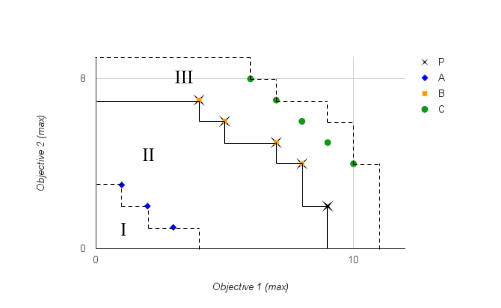
\includegraphics[width=.7\textwidth]{../images/BinaryEpsilonIndicator}
\caption[The additive binary epsilon indicator $I_{\epsilon_+2}$]{Depiction of the additive binary epsilon indicator $I_{\epsilon_+2}$ and the additive epsilon dominance relationship $\succeq_{\epsilon_+}$. In the figure,

\begin{minipage}{\linewidth}
  \begin{align*}
    I_{\epsilon_+2} (P,A) = -4 < 0 \qquad I_{\epsilon_+2} (P,B) = 0 \qquad I_{\epsilon_+2} (P,C) = 2 > 0
  \end{align*}
\end{minipage}

Region III is $\epsilon_+$-dominated for $\epsilon = 2$; region II is $\epsilon_+$-dominated for $\epsilon = 0$; region I is $\epsilon_+$-dominated for $\epsilon = -4$. Note that region II also encompasses region I, and region III encompasses region II.}
\label{fig:binaryEpsilon}
\end{figure}

\subsection{Additive unary epsilon indicator $I_{\epsilon_+}$} I define the unary epsilon indicator as
\begin{align}
I_{\epsilon_+} (Z) = I_{\epsilon_+2} (Z,\mathbf{z}_{\text{ideal}})
\end{align}
That is, the additive unary epsilon indicator is identical to the additive binary epsilon indicator where the second frontier consists of a single point: the ideal solution for the first frontier.

This differs from the unary epsilon indicator traditionally used in EMO \cite{zitzler2003performance}. In EMO, the frontier is compared against a reference nondominated set. However, because the frontiers in the present study have guaranteed optimality, there is no reference set against which to compare them.

\subsection{Unary hypervolume indicator $I_{H1}$ and binary hypervolume indicator $I_{H2}$}
\label{sec:hypervolumeIndicator}
For every solution $\mathbf{z}_i$ in a frontier $Z$ define the hyperrectangle $r_i$ whose diagonal corners are the origin and the objective vector $\mathbf{z}_i = \braket{z^1,\ldots,z^N}$ (see Figure \ref{fig:frontierVolumes}). Then the unary hypervolume indicator of the frontier $Z$ is the $N$-dimensional volume of the union of all of the hyperrectangles corresponding to the solutions in $Z$:
\begin{align}
I_{H1} (Z) = \text{vol} \left( \bigcup_{i = 1}^{|Z|} r_i \right)
\end{align}
Then define the binary hypervolume indicator of two frontiers $Z_1$ and $Z_2$ as \cite{zitzler1999evolutionary}
\begin{align}
I_{H2} (Z_1,Z_2) = I_{H1} (Z_1 + Z_2) - I_{H1} (Z_2)
\end{align}
where $I_{H1} (Z_1 + Z_2)$ is the unary hypervolume indicator of the frontier consisting of the nondominated points in $Z = \{z \in Z_1 \cup Z_2\}$ . See Figure \ref{fig:binaryHypervolume}. The binary hypervolume indicator provides the volume of frontier $Z_1$ that is not contained within frontier $Z_2$. Larger values of $I_{H1}$ correspond to frontiers occupying larger amounts of the objective space. In a normalized objective space, $I_{H2}(Z_1, Z_2) > I_{H2}(Z_2, Z_1)$ indicates areas of less conflict between objectives in $Z_1$ than in $Z_2$.

\begin{figure}[ht]
\centering
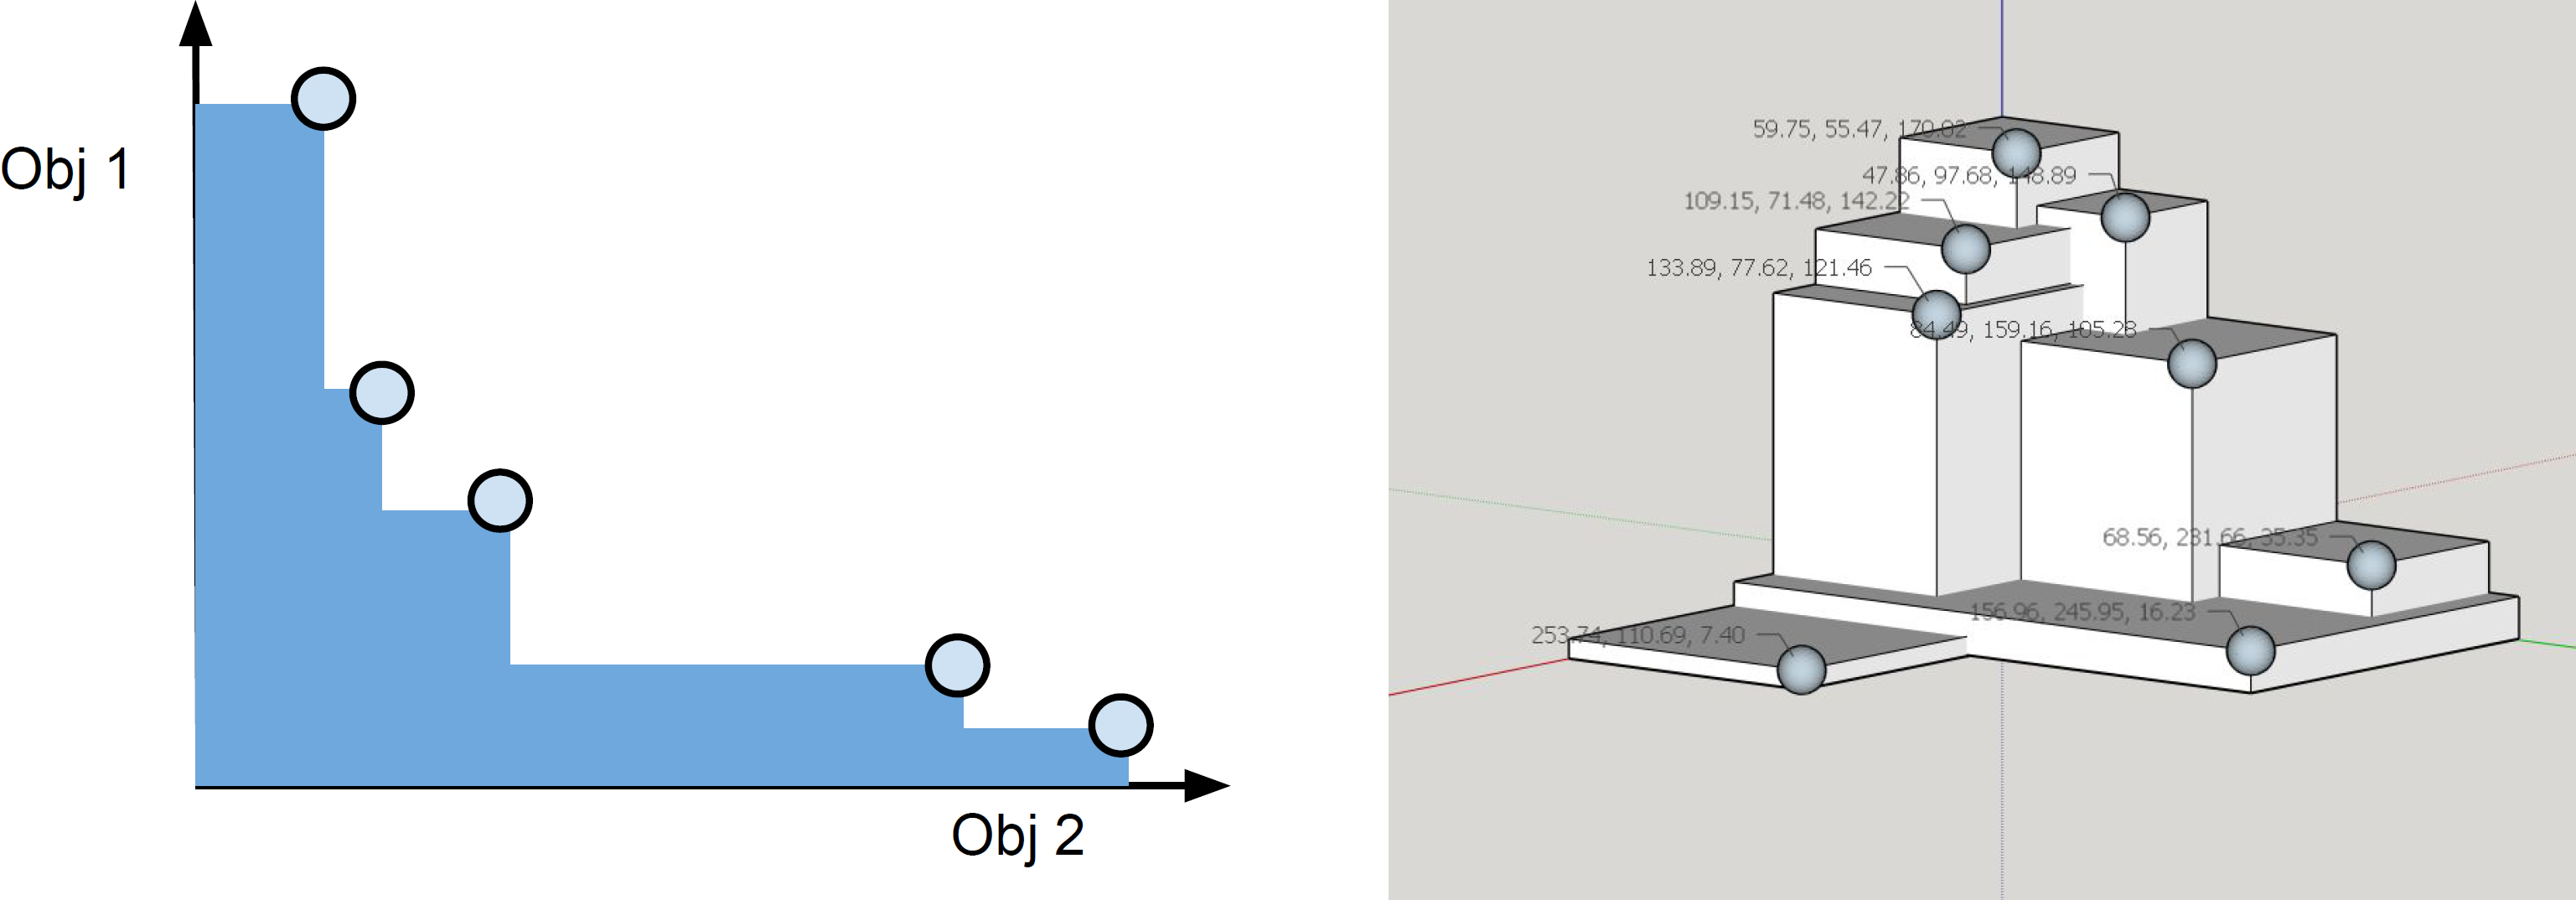
\includegraphics[width=.85\textwidth]{../images/FrontierVolumesNo2DOutlines}
\caption[Hypervolume of Pareto frontiers]{Depiction of the hypervolumes of frontiers with two objectives (left) and three objectives (right).}
\label{fig:frontierVolumes}
\end{figure}

\begin{figure}[ht!]
\centering
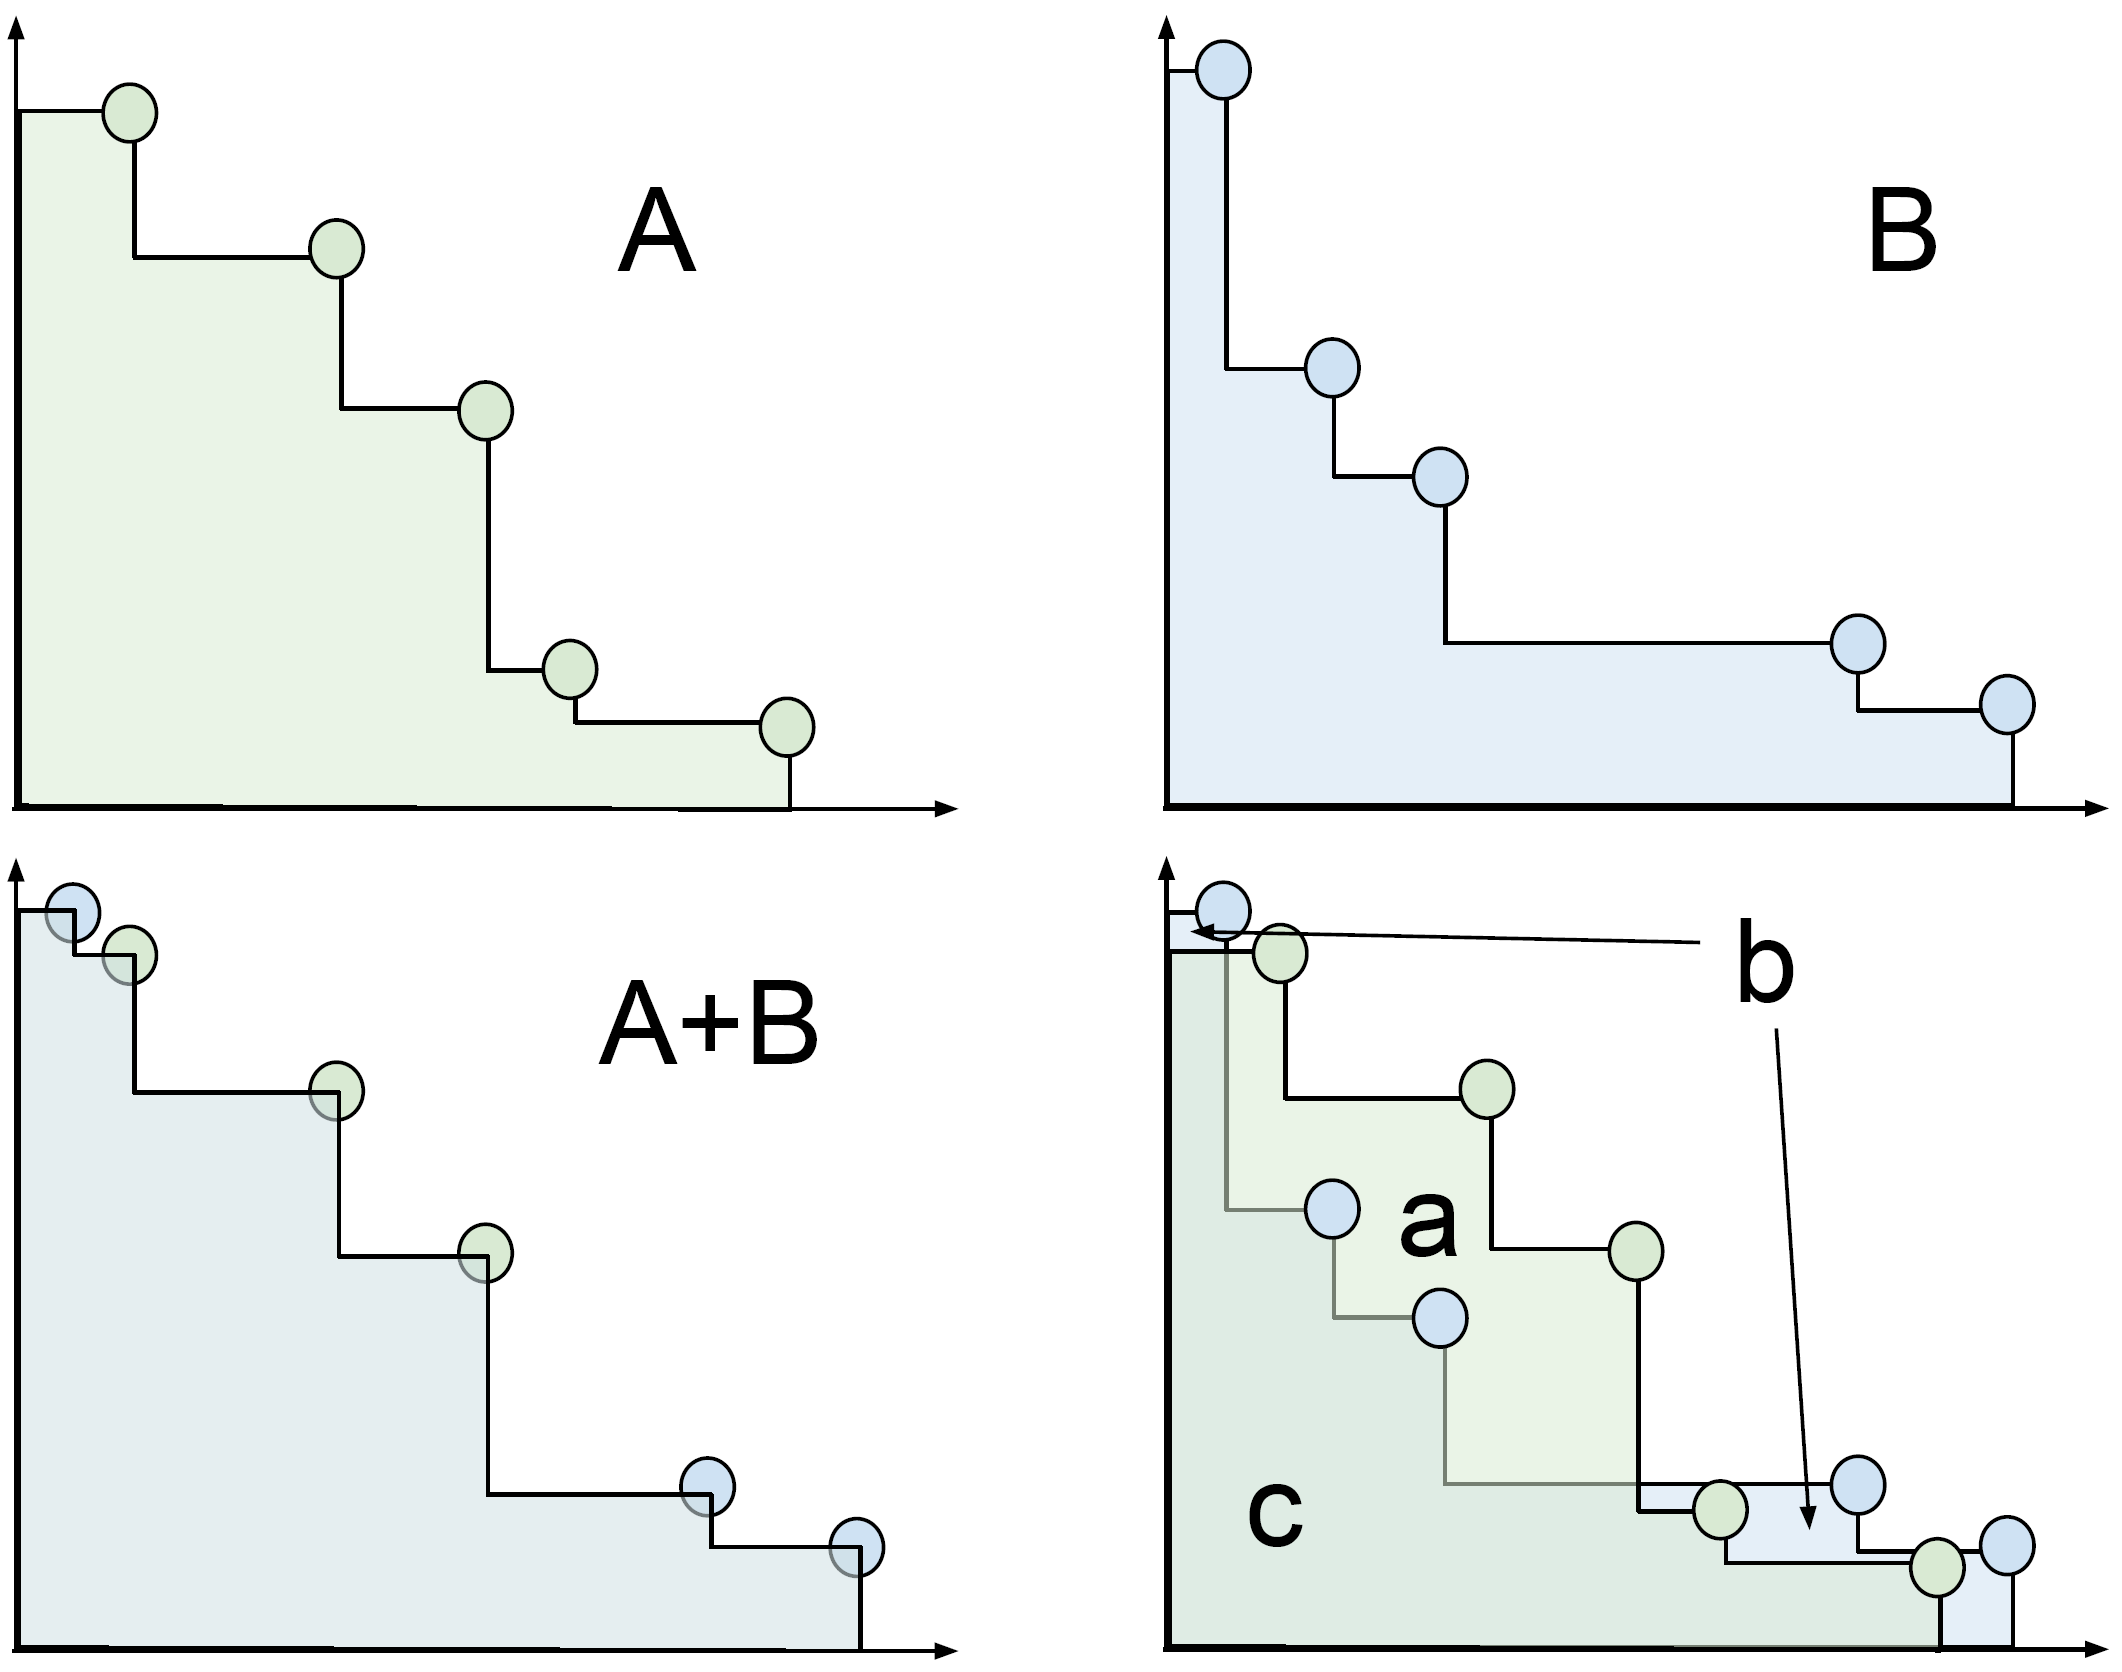
\includegraphics[width=.7\textwidth]{../images/BinaryHypervolume}
\caption[Binary hypervolume indicator]{Depiction of the binary hypervolume indicator. The individual frontiers are shown in the top row: frontier $A$ (left) and frontier $B$ (right). The merged frontier $A+B$ is shown in bottom left - note the absence of points that were dominated when combined. Following the naming of regions as shown in the bottom right figure, the binary hypervolume indicator is equal to
\begin{minipage}{\linewidth}
  \begin{align*}
    I_{H2} (A,B) = \left(\text{area}_a + \text{area}_b + \text{area}_c \right) - \left( \text{area}_b + \text{area}_c \right) = \text{area}_a
  \end{align*}
\end{minipage}%
}
\label{fig:binaryHypervolume}
\end{figure}

I developed a custom algorithm to solve for the hypervolume idicators. The details of the algorithm may be found in \S \ref{chap:appAHypervolumeAlgo}.

\subsection{Unary distance indicator $I_d$} The unary distance indicator measures the average distance from the frontier to the ideal solution:
\begin{align}
I_d = \frac{\sum_{\mathbf{z} \in Z} ||\mathbf{z}_{\text{ideal}} - \mathbf{z} ||}{N}
\end{align}
Smaller values of $I_d$ correspond to frontiers that are closer to the ideal solution, which may imply less conflict between objectives. This metric is analogous to the unary distance indicator more commonly used in EMO \cite{czyzzak1998pareto}. Where the metric used here measures the distance to the ideal solution, the traditional metric measures the distance to a reference Pareto frontier.

\subsection{Unary Spacing Indicator $I_s$} The unary spacing indicator, or Schott's spacing metric \cite{schott1995fault}, computes the standard deviation of the distance between points in the frontier:
\begin{align}
I_s = \sqrt{\frac{1}{N-1} \sum_{\mathbf{z} \in Z} (d_z - \overbar{d})^2}
\end{align}
where
\begin{align}
d_z = \min_{\mathbf{y} \in Z, \mathbf{y} \neq \mathbf{z}} ||\mathbf{z} - \mathbf{y}||
\end{align}
and $\overbar{d}$ is the average over all $d_z$. In EMO, the spacing indicator provides a measure of an algorithm's ability to search the frontier space uniformly. Here, the spacing metric provides a measure of the flexibility afforded to the decision maker under each climate scenario, since smaller values of $I_s$ imply a higher density of solutions and greater flexibility.

\section{Intra-Frontier Comparison Metrics}
\label{sec:withinFrontierMetrics}
While the above methods provide frontier-level metrics of conflict and tradeoffs, there are two methods employed here to also determine the degree of conflict within a single frontier. The first is an approach used in many-objective optimization, and the second is a variant of the unary hypervolume indicator.

\subsection{Pearson correlation coefficients} Given the increased difficulty in solving many-objective optimization problems \cite{khare2003performance}, researchers in this field seek to reduce the number of objectives considered in the model. To determine which objectives most strongly influence the shape of the frontier, they compute the correlation between each pair of objectives \cite{deb2005finding}. Objective pairs with strong negative correlation conflict with one another. The Pearson correlation coefficients are computed per
\begin{align}
\rho_{X,Y} = \frac{\text{cov}(X,Y)}{\sigma(X)\sigma(Y)}
\end{align}
where, for objectives $x$ and $y$, $X$ and $Y$ are
\begin{align}
X = \{ \mathbf{z}^x_1, \mathbf{z}^x_2, \ldots, \mathbf{z}^x_{|Z|} \} \\
Y = \{ \mathbf{z}^y_1, \mathbf{z}^y_2, \ldots, \mathbf{z}^y_{|Z|} \}
\end{align}

\subsection{Area of 2D frontier projection $A_{xy}$}
The second intra-frontier comparison metric uses the unary hypervolume indicator described in \S \ref{sec:hypervolumeIndicator}. Given a frontier with objective vectors in $N$ dimensions, take two objectives $x$ and $y$, and project the $N$-dimensional frontier to the two-dimensional $xy$-plane. Remove solutions dominated in this projection, and compute the hypervolume indicator (which, in two-dimensions, is simply the area). See Figure \ref{fig:frontierCrossSection}. Larger values of $A_{xy}$ imply less conflict between objectives $x$ and $y$.

\begin{figure}[ht]
\centering
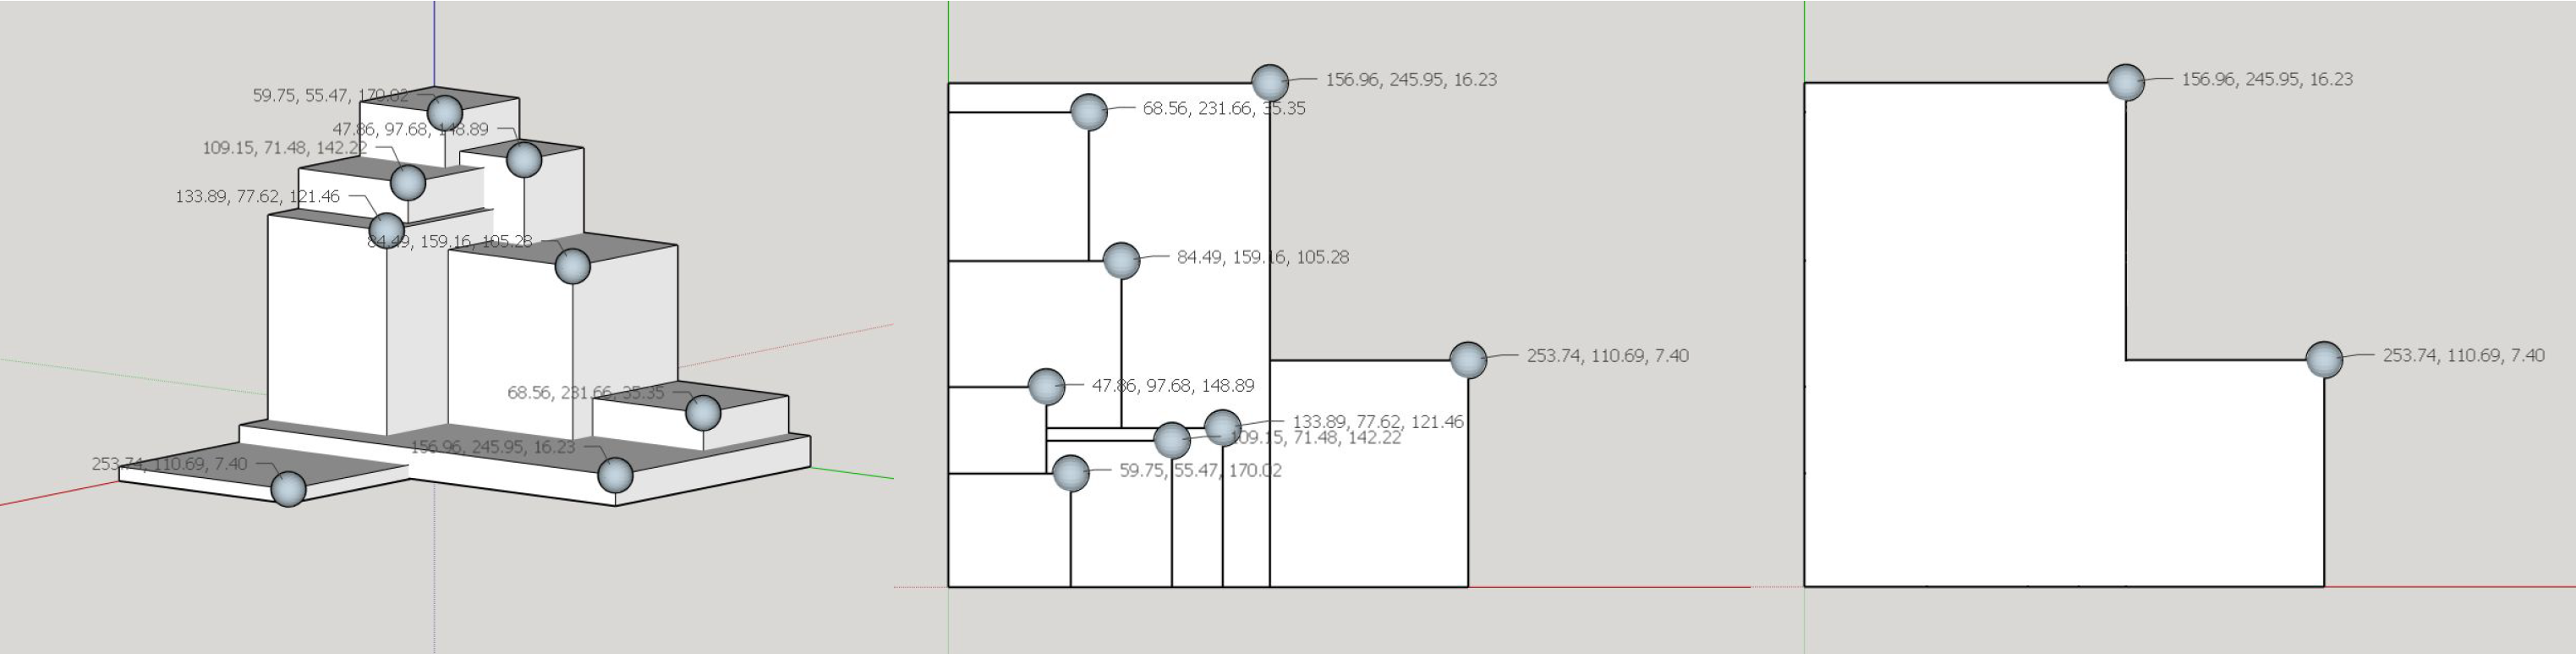
\includegraphics[width=\textwidth]{../images/CrossSection2D}
\caption[Area of 2D frontier projection]{Comparing conflict between objectives based on the area bounded by two-dimensional frontier projection. Left is the original frontier; middle shows the 2D projection of the frontier; right shows the projected frontier with all dominated solutions removed. Assuming both objectives are maximized, the larger the area bounded by the cross-sectional area, the less conflict between the objectives.}
\label{fig:frontierCrossSection}
\end{figure}